\documentclass{article}
\usepackage{graphicx}
\usepackage[margin=1in]{geometry}
\usepackage[dvipsnames]{xcolor}
\usepackage{lipsum}
\usepackage[backend=biber,style=apa]{biblatex}
\addbibresource{bibliography.bib}  % Make sure this is the correct path
\usepackage{amsmath}
\usepackage{listings}  % For code listings
\usepackage{xcolor}    % For syntax highlighting
\usepackage[utf8]{inputenc}
\usepackage{subcaption}
\usepackage{float}  % Add this in the preamble for the [H] specifier




\title{Project report (PRA2003)}
\author{Your name}
\date{\today}

\begin{document}



\begin{titlepage}
    \begin{center}
        
\includegraphics[width=8cm]{lab report/MSP-logo.jpg} 
        \vspace{1cm}
        
        \textbf{\LARGE Matter--antimatter asymmetry in PYTHIA:}\\
        \textbf{\LARGE Focus on pion\textbf{}}
        
        \vspace{1.5cm}
        
        \textbf{\Large Papot Clotilde}
        \vfill
        \large Date: \today
        
    \end{center}
\end{titlepage}

\newpage
\section*{Introduction}

In the quest of understanding the origin of universe, scientists elaborated the Big Bang Theory. This theory suggests that at the universe's inception, both matter and antimatter were created. However, we observe that, in our current universe, everything is made of matter. So, where did antimatter go? (\cite{robson2018}) 
\\

To address this question, we must first understand what antimatter is and how it interacts with matter. Antimatter is considered the mirror image of matter, while both share the same properties, like mass, they have opposite charges. For each particle in the universe, there exists its corresponding antiparticle: electrons have positrons as their corresponding antiparticle, in the same way that protons have instead antiprotons. When matter and antimatter interact, they annihilate each other (\cite{cern_matter_antimatter_asymmetry}).
\\

Scientists suspect there was an asymmetry in the amount of matter and antimatter in the early stage of our universe. After most of the matter and antimatter annihilated each other, a small excess of matter remained. This imbalance caused matter to prevail over antimatter, leading to the creation of all the things that surrounds us today and the absence of antimatter (\cite{cern_matter_antimatter_asymmetry}). The existence of this asymmetry is what researchers are still trying to prove.
\\

Recent technologies, such as particle accelerator, offer new opportunities to explore this question. Particle accelerators are used to facilitate collision between particles (like protons). These protons are accelerated in opposite directions in a large circular structure, thanks to electrical fields. They can reach extremely high speed (near the speed of light), allowing an enormous release of energy when they collide. This energy is then available to produce new particle of matter and antimatter (\cite{DOE2024}).
\\  

These accelerators allow scientists to study particles that are not commonly found, like pions, which are the focus of this paper.
Pions, also known as pi mesons, are composed of quarks and anti-quarks and are among the lightest mesons. Positive pions are made of an up quark and an anti-down quark, while negative pions are made of a down quark and an anti-up quark. They are antiparticles of each other. Pions are known for their role in mediating the strong nuclear force, which binds protons and neutrons together in atomic nuclei. (\cite{pasayten2021})
\\

This paper will investigate whether there is an asymmetry of matter and antimatter produced following protons collision. To do so, we will analyze data samples from a model, PYTHIA, which simulates these kinds of collisions, as we unfortunately did not have access to a particle accelerator. As mentioned, we will focus on pions. More specifically, we will investigate momentum of positive and negative pions. 




\section*{Analysis details}
%No more than half a page including tables or/and figures

As mentioned in the introduction, the data used for this analysis was gathered from PYTHIA. The dataset consists of 10 files of each 500000 events, which contain the recorded momentum of each particle produced by the proton-protn collision in the x, y and z direction. It also include PDG codes. The PDG code is an integer identifying uniquely each type of particle. 
\\
\\
Since this paper focuses on pions, only the data corresponding to the PDG codes 211 (for positive pions) and -211 (for negative pions) were selected. This selection and all subsequent calculations were performed using two pythons scripts specifically developed for this analysis.  
\\
\\
The first script analyzed the entire dataset and computed the amount of matter and anti-matter produced by the collision. It calculated the average number of positive and negative pions across all files using a subsampling method, where each file served as a subsample. 
\\
\\
First the average amount of positive and negative pions per event was calculated for each file. Then using these values, an overall weighted average for both type of pions was conducted (the weigth being the number of events per file). The standard deviation of the averages per event per file was used to estimate the uncertainties of the overall averages.
\\
\\
Additionally, the mean differences between the average number of positive and negative pions per events was calculated for each file, followed by the overall average of these mean differences. The corresponding uncertainty of this overall average was again established using the standard deviation between the mean differences of each file. 
\\
\\
The second python script computed several parameters on the whole data set, such as the total momentum, the pseudo-rapidity and the transversal momentum of each pions particle. These values provide critical information on the spatial distribution and energy levels of the different particles resulting from the collision. Analyzing these parameters is essential to investigate the hypothesis. Significant discrepancies between the results for positive and negative pions would suggest such asymmetry. The different calculations where conducted as follows:
\\
The total momentum (p) (in GeV/c) was computed using this formula:

\[p = \sqrt{p_x^2 + p_y^2 + p_z^2} \quad \text{(\cite{Christakoglou2024})}\]

The pseudo-rapidity ($\eta$) (dimensionless) was computed using this formula:

\[\eta = \frac{1}{2} \ln{\left( \frac{p + p_z}{p - p_z} \right)}\quad \text{(\cite{Christakoglou2024})}\]

The transverse momentum (pT) (in GeV/c) was computed using this formula:

\[pT=\sqrt{px^2+py^2+}\quad \text{(\cite{Christakoglou2024})}\]


After calculating these parameters for both positive and negative pions accross all files, the code sorted these values into different bins based on pseudorapidity and for transverse momentum. The number of positive and negative pions falling within each ranges was then counted. These counts were normalised per event by dividing them by 5,000,000, the total number of events across all file. Uncertainties for these counts were computed using the Poisson error method, where the square root of the count was divided by the total number of events.
\\
\\
Additionally, the difference between the normalized counts of positive and negative pions within each bin (for both pseudorapidity and transverse momentum) was calculated by subtracting the normalized count of negative pions from that of positive pions. The uncertainties for these differences were determined using the subsampling method, with the 10 files serving as subsamples. To do so, the normalised differences per bins were calculated for each file. The standard deviation across the subsamples was then used to represent the uncertainties for each bins. This approach allowed for the creation of histograms describing the pion distributions as a function of pseudorapidity and transverse momentum, facilitating the comparison between the number of positive and negative pions across these variables. 
\\



\section*{Results}

The results of the calculations performed by the two Python scripts are summarized in the following tables. The first script analyzed the overall average number of pions produced by the collisions for each events and their difference.
The second script calculated the number of positive and negative pions in function of pseudorapidity and transverse momentum, as well as the differences between pions and anti-pions.
\\

Table 1 presents the results for the average number per event of both positive and negative pions produced by the collisions. The mean difference between positive and negative pions is also displayed.
7,5
\begin{table}[ht]
    \centering
    \caption{Average Amount of Positive and Negative Pions}
    \begin{tabular}{|l|c|c|}
        \hline
        Pion Type                      & {Average Amount}       & {Uncertainty}         \\ \hline
        Positive Pions                 & 18.43                & ± 0.03             \\ \hline
        Negative Pions                 & 18.40                & ± 0.03              \\ \hline
        Difference of Means            & 0.030                 & ± 0.004            \\ \hline
    \end{tabular}
\end{table}
\newpage
Graphs (a) and (b) display the number of pions (in blue) and anti-pions (in orange) per event, along with their corresponding uncertainties, as a function of pseudorapidity and transverse momentum ranges, respectively.

\begin{figure}[H]
  \centering
  % First row with Figures 1 and 2
  \begin{subfigure}{0.49\textwidth}
    \centering
    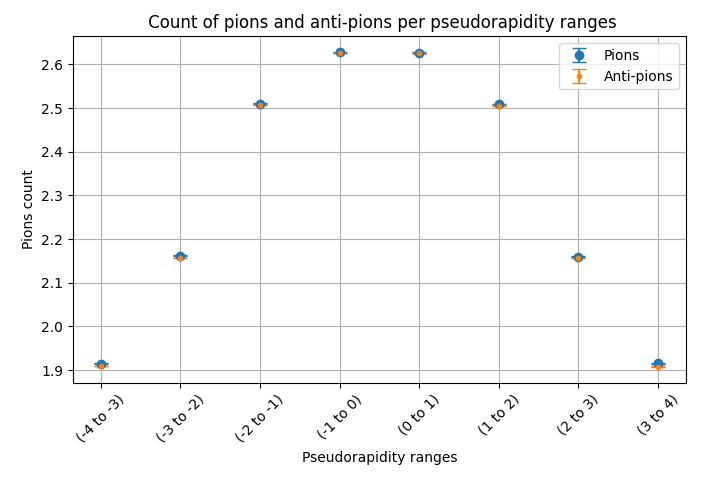
\includegraphics[width=\linewidth]{lab report/Figure_1_final.png}
    \caption{Count of pions as a function of pseudorapidity}
    \label{fig:subfig1}
  \end{subfigure}
  \hfill
  \begin{subfigure}{0.49\textwidth}
    \centering
    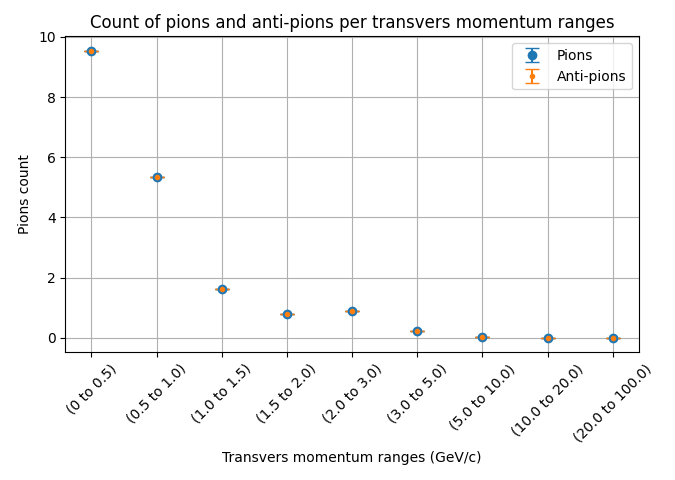
\includegraphics[width=\linewidth]{lab report/Figure_2_final.png}
    \caption{Count of pions as a function of transverse momentum}
    \label{fig:subfig2}
  \end{subfigure}
  
  \vskip\baselineskip  % Adds vertical space between rows
  
  % Second row with Figures 3 and 4
  \begin{subfigure}{0.49\textwidth}
    \centering
    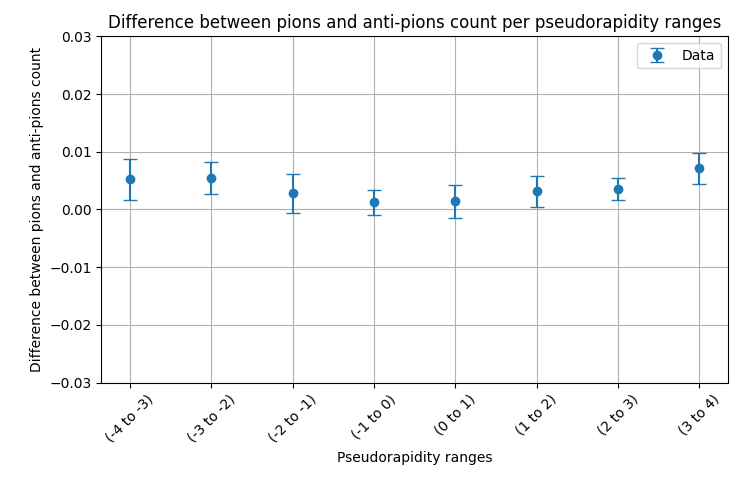
\includegraphics[width=\linewidth]{lab report/Figure_3_final.png}
    \caption{Difference in pion count as a function of pseudorapidity}
    \label{fig:subfig3}
  \end{subfigure}
  \hfill
  \begin{subfigure}{0.49\textwidth}
    \centering
    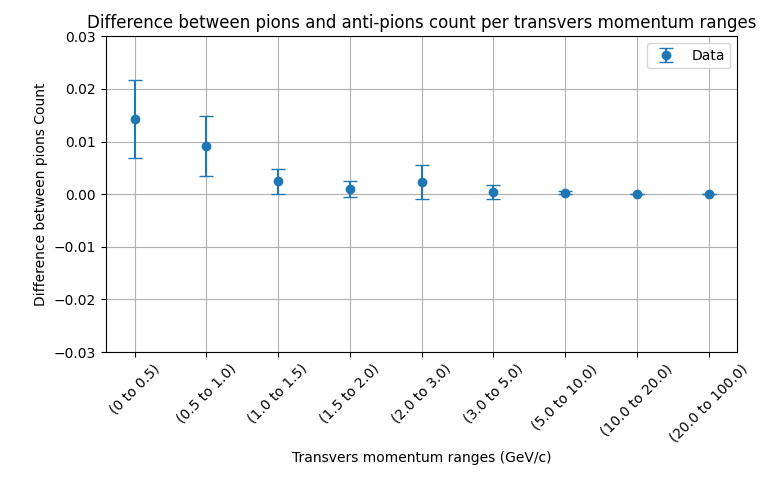
\includegraphics[width=\linewidth]{lab report/Figure_4_final.png}
    \caption{Difference in pion count as a function of transverse momentum}
    \label{fig:subfig4}
  \end{subfigure}
\end{figure}


\section*{Discussion}
The different graph (graph (a) and (b)) presented in the result section show that the number of postive and negative pions as function of pseudorapidity and transvers momentum are quite similar. This resemblance could initially suggest a symmetry between them. 
\\

However, the difference graphs (graph (c) and (d)) show that the differences do not equal zero in certain bins, indicating potential asymmetry in those ranges. 

Moreover, the trend observed in graph(d), of increasing differences in lower pt ranges(0 to 1.5 GeV/c) compared to higher ranges suggest that PYTHIA may treat the creation of particles and antiparticles differently as a function of energy. In this context, lower energy appears to correlate with a higher production rate of pions relative to anti-pions. Similarly for pseudorapidity, the observed trend in graph (c) shows increasing differences in lower $\eta$ ranges (-4 to -1) as well as in higher ranges (1 to 4). This might imply that the mechanisms PYTHIA use for governing their pion production can be influenced by the angle of emission relative to the collision axis. This suggests that certain angles, particularly those further from the beam axis, may favor the production of pions over anti-pions.
\\

However before drawing conclusions, the significance of the results need to be evaluated. This involves determining how many standard deviation ($\sigma$) the values are from the reference point, which is a mean difference of zero representing the null hypothesis of no asymmetry. The number of $\sigma$ can be found by comparing the mean difference to its associated uncertainty using the following formula:

\[\frac{\text{mean difference}}{\text{uncertainty}}\approx n \sigma\]

Applying this formula to the mean differences per bin of pseudorapidity and transverse momentum (as shown in graph (c) and (d)) yield $\sigma$ ranges from 0.48$\sigma$ to  2.61$\sigma$ for pseudorapidity and from 0.29$\sigma$ to  1.92$\sigma$ for transverse momentum. None of the values are above the 3$\sigma$ threshold (indicating statistical significance at a 99.7\% confidence level, the common minimum required to draw any conclusion), meaning that the results per bins are not statistically significant. This weakens the suggested asymmetry, as the observed differences could be due to random fluctuations. It is important to note that non-significant results don't prove symmetry; they indicate that no definitive conclusion can be made from the current data. Further investigation are needed to assess the effects of pseudorapidity and transverse momentum on pions anti-pions production.    
\\

While the pseudorapidity and transvers momentum results fail to show significance, the analysis of the pion counts present a different outcome. Similarly, the significance of the mean difference between the number of positive and negative pions (as shown in table 1) can be determined. Using the previous formula, the number of sigma found for this result is $\approx$ 7.5$\sigma$. This means the value is highly significant, as it largely exceed the 3$\sigma$ threshold. Even though the difference is really small, the high significance suggest that indeed there is more matter than anti matter following the collision of protons. Thereby this result support the hypothesis of this paper.
\\

In conclusion, the analysis indicates that the overall averages of pion and anti-pion production support the hypothesis of matter-antimatter asymmetry following proton collisions, implying that PYTHIA captures fundamental trends, such as a slight excess of matter over antimatter. However, the lack of statistical significance in the differences based on pseudorapidity and transverse momentum suggests that these factors may not be responsible for the observed asymmetry, or that PYTHIA may oversimplify these aspects of particle interactions. Consequently, future experiments are necessary to further investigate this topic, potentially focusing on different collision energies, particle types, or refining the modeling approaches to better understand the dynamics of matter-antimatter production.


%\section*{Conclusion}
%No more than half a page


\printbibliography

\end{document}